\documentclass[a4paper]{article}
% Shared preamble for the English probability and statistics documents.
% Based on the original course preamble. Compile with pdfLaTeX.
\usepackage[top=1.5cm,bottom=2cm,left=2cm,right=2cm]{geometry}
\usepackage[T1]{fontenc}
\usepackage{lmodern}
\usepackage[utf8]{inputenc}
\usepackage[english]{babel}

\usepackage{amsmath}
\usepackage{amssymb}
\usepackage{amsthm}
\usepackage{mathrsfs}
\usepackage{mathtools}
\usepackage{etoolbox}
\usepackage{tikz}
\usetikzlibrary{shapes.multipart,arrows.meta}
\usepackage{xcolor}
\usepackage{enumerate}
\usepackage[shortlabels]{enumitem}
\usepackage{hyperref}
\usepackage{version}
\usepackage{bbold}
\usepackage{fontawesome5}
\usepackage{fancyhdr}
\lfoot{}
\usepackage{natbib}
\usepackage{graphicx}
\usepackage{pdfpages}
\usepackage{authblk}
    
\usepackage{blindtext}
\usepackage{multicol}
\usepackage{collcell}
\usepackage{wrapfig}
\usepackage{blkarray}
\usepackage{cancel}
\usepackage{appendix}
\usepackage{float}
\makeatletter
\input{tex/assets/slashbox.sty}
\makeatother
\hypersetup{unicode,colorlinks,citecolor=red,filecolor=black,
  linkcolor=red,urlcolor=cyan}
\setlength{\columnsep}{1cm}
\pagenumbering{gobble}

\def\numtext#1{%
  \ifcase#1\or one\or two\or three\or four\or five\or six\or seven\or eight\or nine\or ten\or
  eleven\or twelve\or thirteen\or fourteen\or fifteen\or sixteen\or seventeen\or eighteen\or nineteen\or twenty\or Lots\fi}

\newcommand{\Byte}[1]{%
  \def\nodecontents{}%
  \foreach[count=\l] \k in {#1} {\xappto{\nodecontents}{\noexpand\nodepart{\numtext{\l}}\k}}%
  \node[rectangle split,rectangle split parts=8,rectangle split horizontal,draw] at (2,2){\nodecontents};}

\newcommand{\D}{{\mathrm{d}}}
\newcommand{\cE}{{\mathcal{E}}}
\newcommand{\cG}{{\mathcal{G}}}
\newcommand{\cX}{{\mathcal{X}}}
\newcommand{\cY}{{\mathcal{Y}}}
\newcommand{\cB}{{\mathcal{B}}}
\newcommand{\cF}{{\mathcal{F}}}
\newcommand{\cO}{{\mathcal{O}}}
\newcommand{\cS}{{\mathcal{S}}}
\newcommand{\cT}{{\mathcal{T}}}
\newcommand{\given}{\, \big| \,}
\newcommand{\cL}{{\mathscr{L}}}
\newcommand{\cD}{{\mathcal{D}}}
\newcommand{\cA}{{\mathscr{A}}}
\newcommand{\cP}{{\mathscr{P}}}
\newcommand{\cR}{{\mathscr{R}}}
\newcommand{\A}{{\mathcal A}}
\newcommand{\one}{\mathbb{1}}
\newcommand{\mathbbm}[1]{\mathbb{#1}}

\providecommand{\C}{}
\renewcommand{\C}{\mathbb C}
\newcommand{\R}{\mathbb R}
\newcommand{\Q}{\mathbb Q}
\newcommand{\N}{\mathbb N}
\newcommand{\T}{\mathbb T}
\newcommand{\F}{\mathbb F}
\renewcommand{\P}{\mathbb P}
\newcommand{\Z}{\mathbb Z}
\newcommand{\E}{\mathbb {E}}
\newcommand{\Pbb}[1]{\P\left( #1\right)}
\newcommand{\Ebb}[1]{\E\left[ #1\right]}

\newcommand{\lb}{\left (}
\newcommand{\rb}{\right )}
\newcommand{\lbb}{\left [}
\newcommand{\rbb}{\right ]}
\newcommand{\labs}{\left |}
\newcommand{\rabs}{\right |}
\newcommand{\lbrb}[1]{\lb #1 \rb}
\newcommand{\lbbrbb}[1]{\lbb#1\rbb}
\newcommand{\labsrabs}[1]{\labs#1\rabs}
\newcommand{\lbbrb}[1]{\lbb#1\rb}
\newcommand{\lbrbb}[1]{\lb#1\rbb}
\newcommand{\langlerangle}[1]{\langle#1\rangle}
\newcommand{\lbcurly}{\{}
\newcommand{\rbcurly}{\}}
\newcommand{\curly}[1]{\lbcurly#1\rbcurly}
\newcommand{\abs}{\labsrabs}
\newcommand{\ind}[1]{1_{#1}}
\newcommand{\indep}{\perp \!\!\! \perp}
\renewcommand{\d}{\, \mathrm{d}}

\newtheorem{theorem}{Theorem}
\newtheorem{problemCnt}{Lemma}
\theoremstyle{definition}
\newtheorem{problem}[problemCnt]{Problem}
\newtheorem{problembook}[problemCnt]{\faBook \,  Problem}
\newtheorem{problempencil}[problemCnt]{\faPencil* \,  Problem}
\newtheorem{problemstar}[problemCnt]{\faStar\,  Problem}
\newtheorem{problemstarpencil}[problemCnt]{\faStar \, \faPencil* \,   Problem}
\newtheorem{probleminteresting}[problemCnt]{\faSmile[regular] \,   Problem}
\newtheorem{solution}{Solution}

\newcommand{\fwcell}[1]{\makebox[\arraystretch\normalbaselineskip]{$#1$}}
\newenvironment{enumeratei}{\begin{enumerate}[(i)]}{\end{enumerate}}
\newenvironment{enumeratea}{\begin{enumerate}[(a)]}{\end{enumerate}}
\newenvironment{enumeraten}{\begin{enumerate}[\upshape 1.]}{\end{enumerate}}

% Compatibility helpers needed by a few files in the combined archive.
\AtBeginDocument{\noindent{\footnotesize English translation prepared with ChatGPT (OpenAI, GPT-6), 26 October 2026, for translation of the Bulgarian text into English and LaTeX formatting.
The Bulgarian originals remain the reference; translation may contain errors.}\par\smallskip}
\newcommand{\MissingGraphic}[1]{%
  \begin{center}\fbox{\parbox{0.82\linewidth}{\centering Missing source image: \texttt{#1}}}\end{center}}



\setlength{\emergencystretch}{3em}
\allowdisplaybreaks
\begin{document}
\noindent Software Engineering \hfill Test 1, 17.12.2022: solutions
\par\smallskip\hrule\smallskip\noindent

\textit{English transcription of the handwritten solutions. Numbering and calculations follow the handwritten original.}

\section*{1. Dividing couples into teams}
\begin{enumerate}
\item Let $X_1$ count people in team A. Then
\[
X_1\sim\operatorname{Bin}(20,\tfrac12),\qquad \boxed{\E X_1=10}.
\]
Let $X_2$ count couples whose members are in the same team. Then
\[
X_2\sim\operatorname{Bin}(10,\tfrac12),\qquad \boxed{\E X_2=5}.
\]
\item A particular person is in the same team as their partner with probability $1/2$. The expected number of divisions is $\boxed{\E\operatorname{Ge}(\tfrac12)=2}$.
\item All couples stay together with probability $(1/2)^{10}$, so
\[
\boxed{\E\operatorname{Ge}((\tfrac12)^{10})=1024}.
\]
If $X_A,X_B$ count couples in teams A and B, then $X_A\stackrel d=X_B$ and $X_A+X_B=10$, hence $\boxed{\E X_A=5}$.
\end{enumerate}

\section*{2. Dice in the bag}
Let $H_i$ mean that we draw $i$ fair and $2-i$ biased dice; let $A$ mean two sixes in two rolls. Initially,
\[
\P(H_2)=\tfrac14,\quad \P(H_1)=\tfrac12,\quad \P(H_0)=\tfrac14.
\]
The likelihoods are
\[
\P(A|H_2)=(\tfrac16)^2,\quad \P(A|H_1)=0.4\cdot\tfrac16,\quad \P(A|H_0)=(0.4)^2.
\]
Thus
\[
\P(H_2|A)=\frac{(\frac16)^2\frac14}
{(\frac16)^2\frac14+\frac12\cdot0.4\cdot\frac16+\frac14(0.4)^2}
=\frac{25}{289}=(\tfrac5{17})^2.
\]
The handwritten solution leaves $\P(H_1|A)$ unevaluated and gives
\[
\P(H_0|A)=\dots=(\tfrac{12}{17})^2,\qquad
\P(\text{biased die}|A)=\frac{12}{17}\approx70.59\%.
\]
We can also proceed in two stages. Let $A$ now mean drawing a die and rolling six, $H_0$ drawing a fair die, and $H_1$ a biased one:
\[
\P(H_0)=\P(H_1)=\tfrac12,\quad \P(A|H_0)=\tfrac16,\quad \P(A|H_1)=40\%.
\]
Then
\[
\P(H_0|A)=\frac{\frac16\frac12}{\frac16\frac12+\frac25\frac12}
=\frac5{17}\approx29.41\%,\qquad \P(H_1|A)=\frac{12}{17}.
\]
Write these updated hypotheses as $H_0^*,H_1^*$. Then
\[
\P(H_0^*|A)=\frac{\frac16\frac5{17}}{\frac16\frac5{17}+\frac25\frac{12}{17}}
=\frac{25}{169}\approx14.79\%,
\]
and approximately $85.21\%$ for a biased die.

\textit{Generalization.} If we draw $n$ times and roll only sixes, let $H_i$ mean that $i$ fair dice were drawn:
\[
\P(H_i)=\binom ni(\tfrac12)^n,\qquad
\P(A|H_i)=(\tfrac16)^i(\tfrac25)^{n-i}.
\]
Hence
\[
\P(H_n|A)=\frac{(\frac16)^n(\frac12)^n}
{\sum_{i=0}^n\binom ni(\frac12)^n(\frac16)^i(\frac25)^{n-i}}
=\frac{(\frac16)^n}{(\frac{17}{30})^n}=(\tfrac5{17})^n.
\]
The notes ask: $\P(\text{fair die})=5/17$?!
This is a procedure for updating beliefs after a new draw.

\section*{3. Penalty shootout}
\begin{enumerate}
\item In each of the first five rounds, both teams must score or both miss:
\[
(75\%\cdot80\%+25\%\cdot20\%)^5\approx11.6\%.
\]
\item Goals in the first five rounds are $X\sim\operatorname{Bin}(5,80\%)$ for team 1 and $Y\sim\operatorname{Bin}(5,75\%)$ for team 2. Thus
\[
\P(X=Y)=\sum_{k=0}^5\P(X=Y=k)
=\sum_{k=0}^5\binom5k^2(75\%\cdot80\%)^k(25\%\cdot20\%)^{5-k}=0.2984.
\]
The probability of a tie after ten rounds is
\[
\P(X=Y)(75\%\cdot80\%+25\%\cdot20\%)^5\approx3.46\%.
\]
\item The handwritten expected-penalty calculation is
\[
10(1-\P(X=Y))+
\P(X=Y)\left(10+\frac1{1-(75\%\cdot80\%+25\%\cdot20\%)}\right)
\approx10.85.
\]
\end{enumerate}

\section*{4. Breaking the segment}
Choose $X_1\sim U(0,1)$ and, conditionally, $Y\sim U(0,1-X_1)$.
Write $Y=(1-X_1)X_2$ with independent $X_1,X_2\sim U(0,1)$.
The three lengths are $X_1,Y,1-X_1-Y$. The triangle inequalities become
\[
\begin{cases}X_1+Y>1-X_1-Y,\\X_1+(1-X_1-Y)>Y,\\Y+(1-X_1-Y)>X_1\end{cases}
\iff
\begin{cases}X_1+Y>\tfrac12,\\Y<\tfrac12,\\X_1<\tfrac12.\end{cases}
\]
Substituting $Y=(1-X_1)X_2$ gives
\[
\begin{cases}X_1+(1-X_1)X_2>\tfrac12,\\(1-X_1)X_2<\tfrac12,\\X_1<\tfrac12\end{cases}
\iff
\begin{cases}X_2>\dfrac{1-2X_1}{2(1-X_1)},\\X_2<\dfrac1{2(1-X_1)},\\X_1<\tfrac12.\end{cases}
\]
The favourable region lies between these curves and left of $X_1=1/2$:
\begin{center}
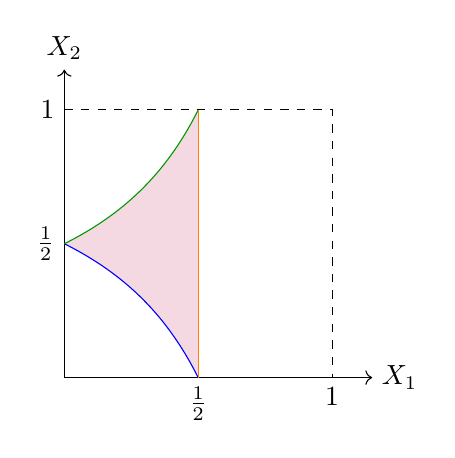
\begin{tikzpicture}[scale=3.4]
\fill[purple!15] plot[domain=0:0.5,samples=50](\x,{1/(2*(1-\x))}) -- plot[domain=0.5:0,samples=50](\x,{(1-2*\x)/(2*(1-\x))}) -- cycle;
\draw[->] (0,0)--(1.15,0) node[right]{$X_1$};
\draw[->] (0,0)--(0,1.15) node[above]{$X_2$};
\draw[dashed] (0,1)--(1,1)--(1,0);
\draw[blue] plot[domain=0:0.5,samples=50](\x,{(1-2*\x)/(2*(1-\x))});
\draw[green!60!black] plot[domain=0:0.5,samples=50](\x,{1/(2*(1-\x))});
\draw[orange] (0.5,0)--(0.5,1);
\node[below] at (0.5,0){$\frac12$};\node[below] at (1,0){$1$};
\node[left] at (0,1){$1$};\node[left] at (0,0.5){$\frac12$};
\end{tikzpicture}
\end{center}
The required area ratio is
\[
\frac{S_{\mathrm{favourable}}}{S_\Omega}
=\frac{\displaystyle\int_0^{1/2}\left(\frac1{2(1-x)}-\frac{1-2x}{2(1-x)}\right)\,dx}{1}
=\int_0^{1/2}\frac{x}{1-x}\,dx=\ln2-\frac12\approx19.32\%.
\]
\end{document}
